\iffalse
Auf der Basis der im vorangegangenen Kapitel erstellten Problemanalyse 
und der im Grundlagenkapitel aufgearbeiteten theoretischen Kenntnisse 
wird ein Lösungskonzept erarbeitet.

Bei Software-Projekten entspricht dieses Kapitel typischerweise der 
Analyse \& Design-Phase des \ac{rup}. Typische Ergebnisse dieser Phase sind 
Klassendiagramme etc.
\fi

% TODO wo soll diese Sektion hin?
\section{Bestehende Visualisierungstools}
\label{sec:bestehende_visualisierungstools}

Es gibt bereits MongoDB Visualisierungtools auf dem Markt, jedoch erfüllt keines davon die zuvor definierten Anforderungen zu genüge:
~\autocite{knowi:mongo_vis_tools}

\subsection{MongoDB Data Explorer}
\label{sub:mongodb_data_explorer}

MongoDB Data Explorer ist ein Tool, welches in MongoDB Atlas integriert ist.
MongoDB Atlas ist ein Web-Tool zur Verwaltung von MongoDB Datenbanken.
Mittels dem MongoDB Data Explorer kann man die Dokumente, Collections und Indexe einer Datenbank anschauen, sowie die Daten mit CRUD Operationen verwalten.
Jedoch bietet der MongoDB Data Explorer keine Möglichkeiten, die Schemas der Dokumente zu analysieren.
\begin{figure}[H]
    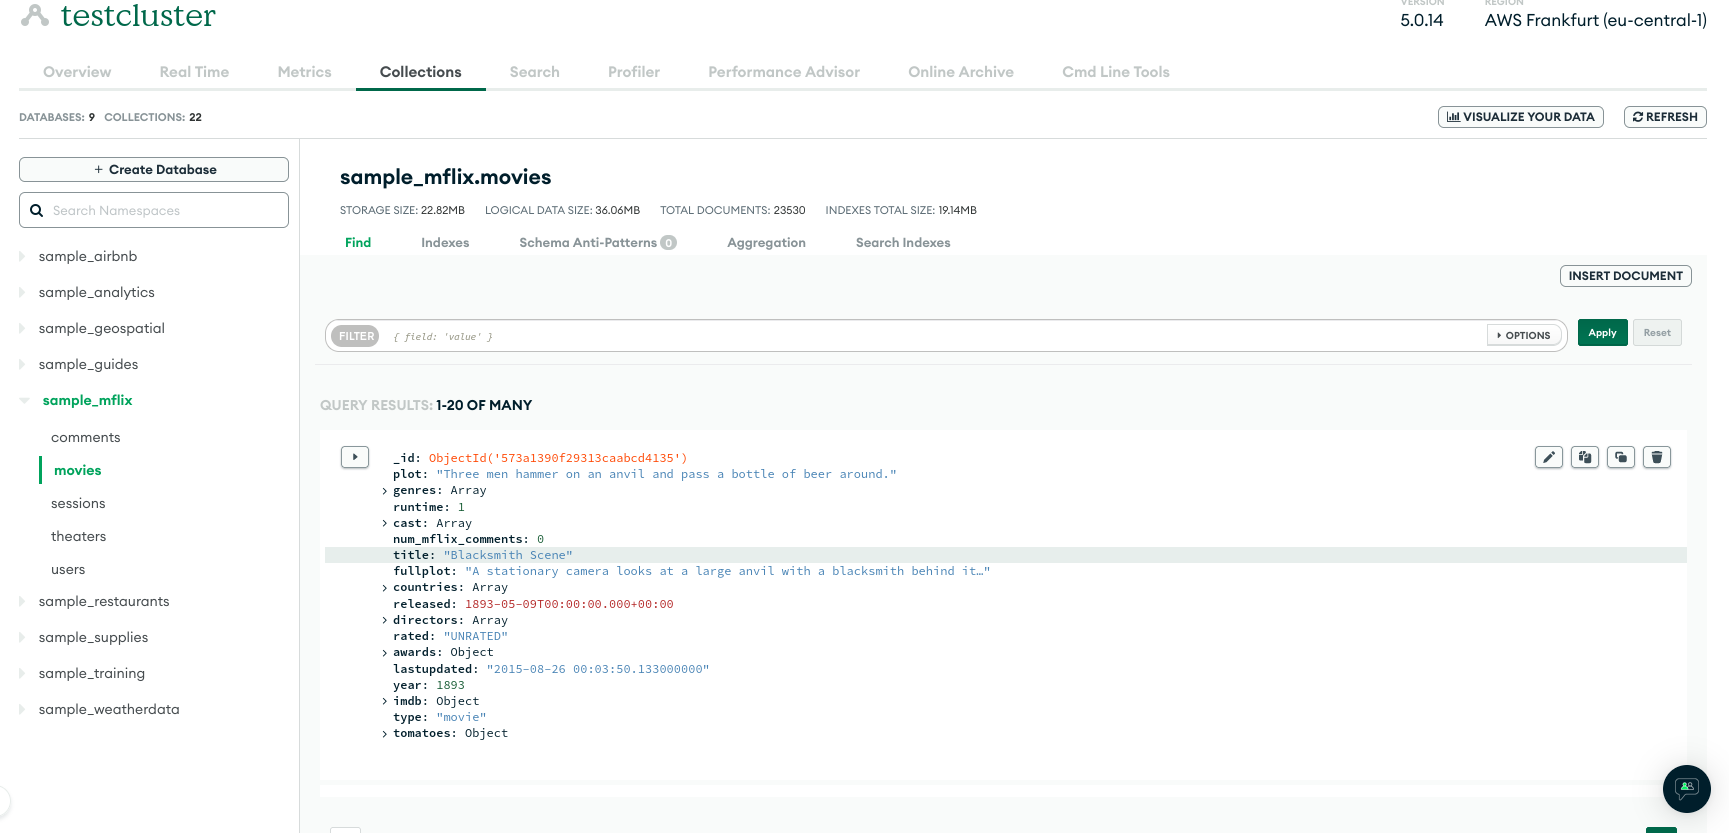
\includegraphics[width=\textwidth]{images/mongodb_data_explorer}
    \caption{MongoDB Data Explorer}
    \label{fig:mongodb_data_explorer}
\end{figure}

\subsection{MongoDB Compass}
\label{sub:mongodb_compass}

MongoDB Compass ist eine Desktop-Anwendung zur Analyse von MongoDB Datenbanken.
MongoDB Compass besitzt ein Schema-Visualisierungstool.
Dieses Schema-Visualisierungstool zeigt sehr genaue Daten zu jedem Feld der Dokumente einer Collection an.
Diese Ansicht ist jedoch nicht besonders übersichtlich, wenn man das gesamte Schema der Dokumente einer Collection analysieren will.
Ebenfalls nicht gut ersichtlich in MongoDB Compass ist die Varianz im Schema zwischen den Dokumenten in einer Collection.
\begin{figure}[H]
    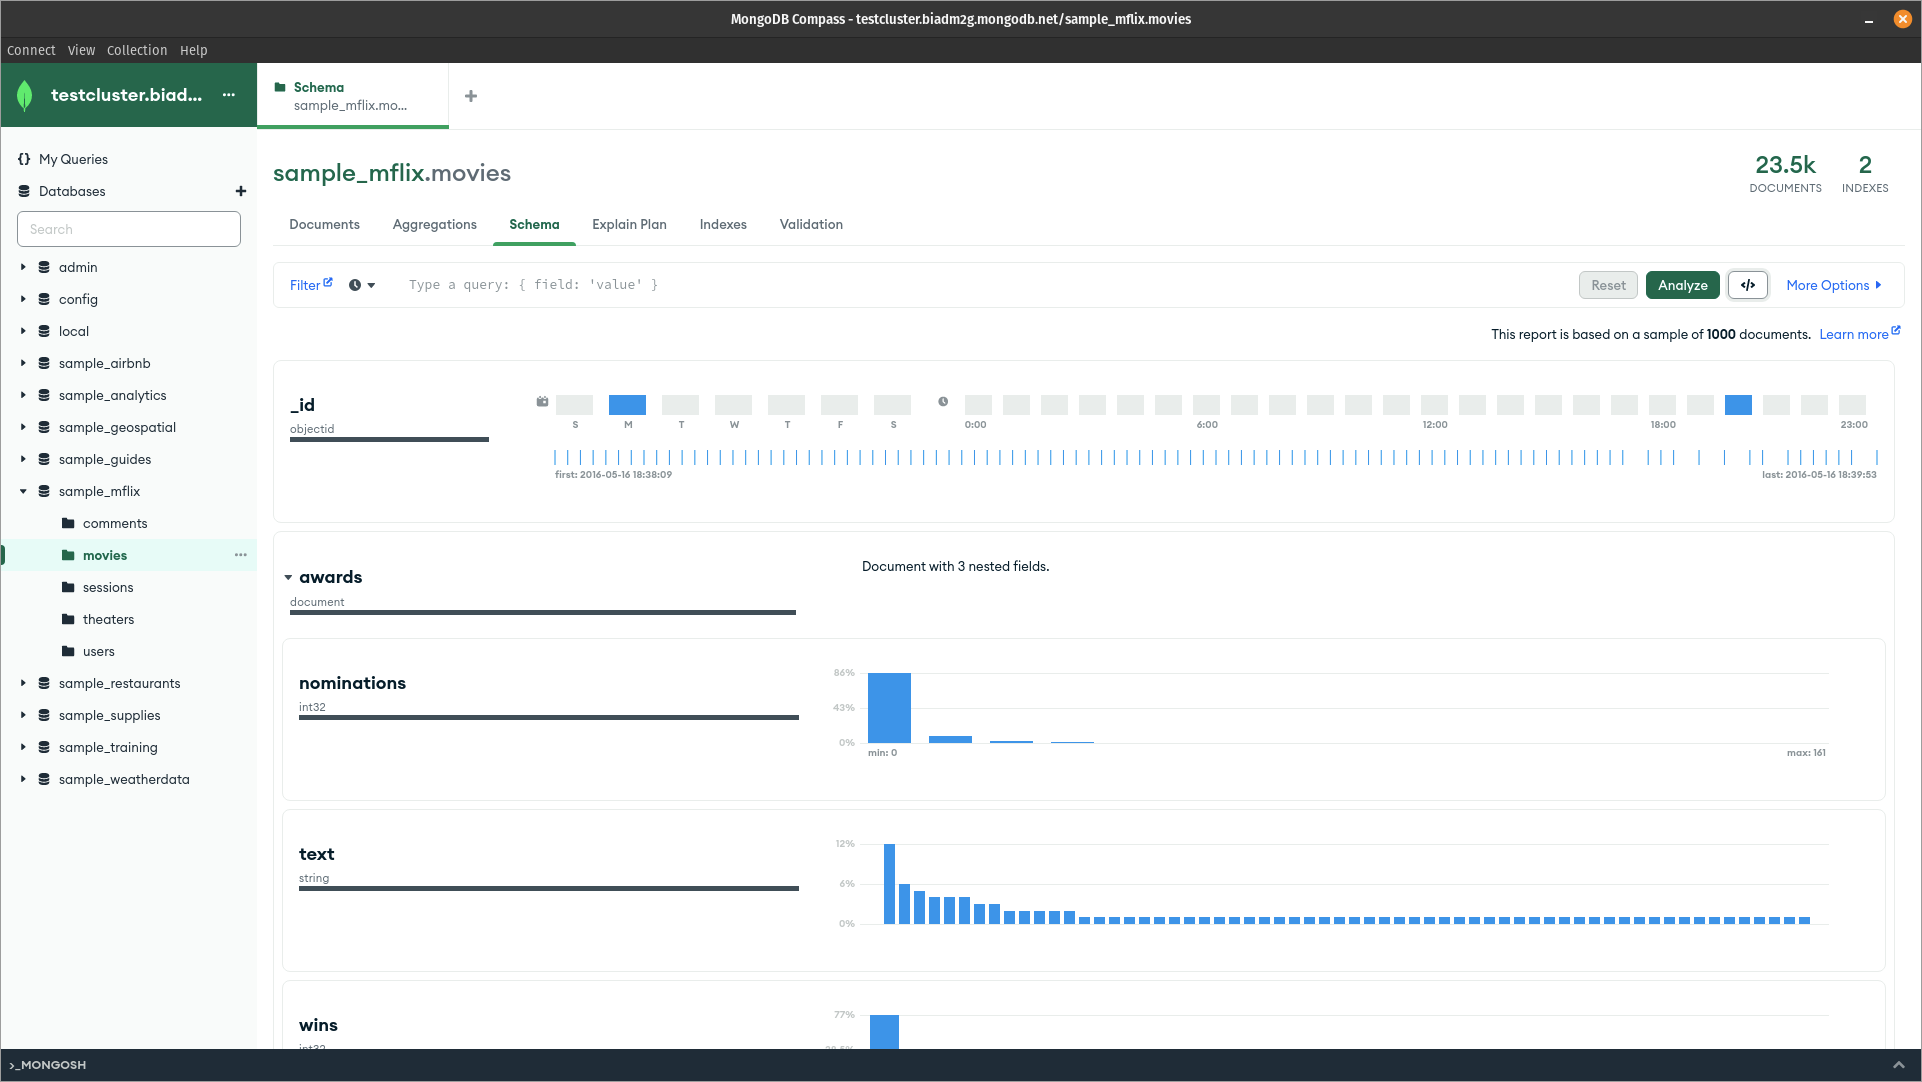
\includegraphics[width=\textwidth]{images/mongodb_compass}
    \caption{MongoDB Compass}
    \label{fig:mongodb_compass}
\end{figure}

\subsection{MongoDB Charts, Tableau, Qlik und Looker}
\label{sub:mongodb_charts}

MongoDB Charts, Tableau, Qlik und Looker sind Tools, die aus MongoDB Daten Graphen generieren und dadurch die Daten in einer MongoDB visualisieren können.
Diese Tools konzentrieren sich jedoch alle auf die Visualisierung der Daten, nicht die Analyse und Visualisierung der Schemas der Dokumente.
\begin{figure}[H]
    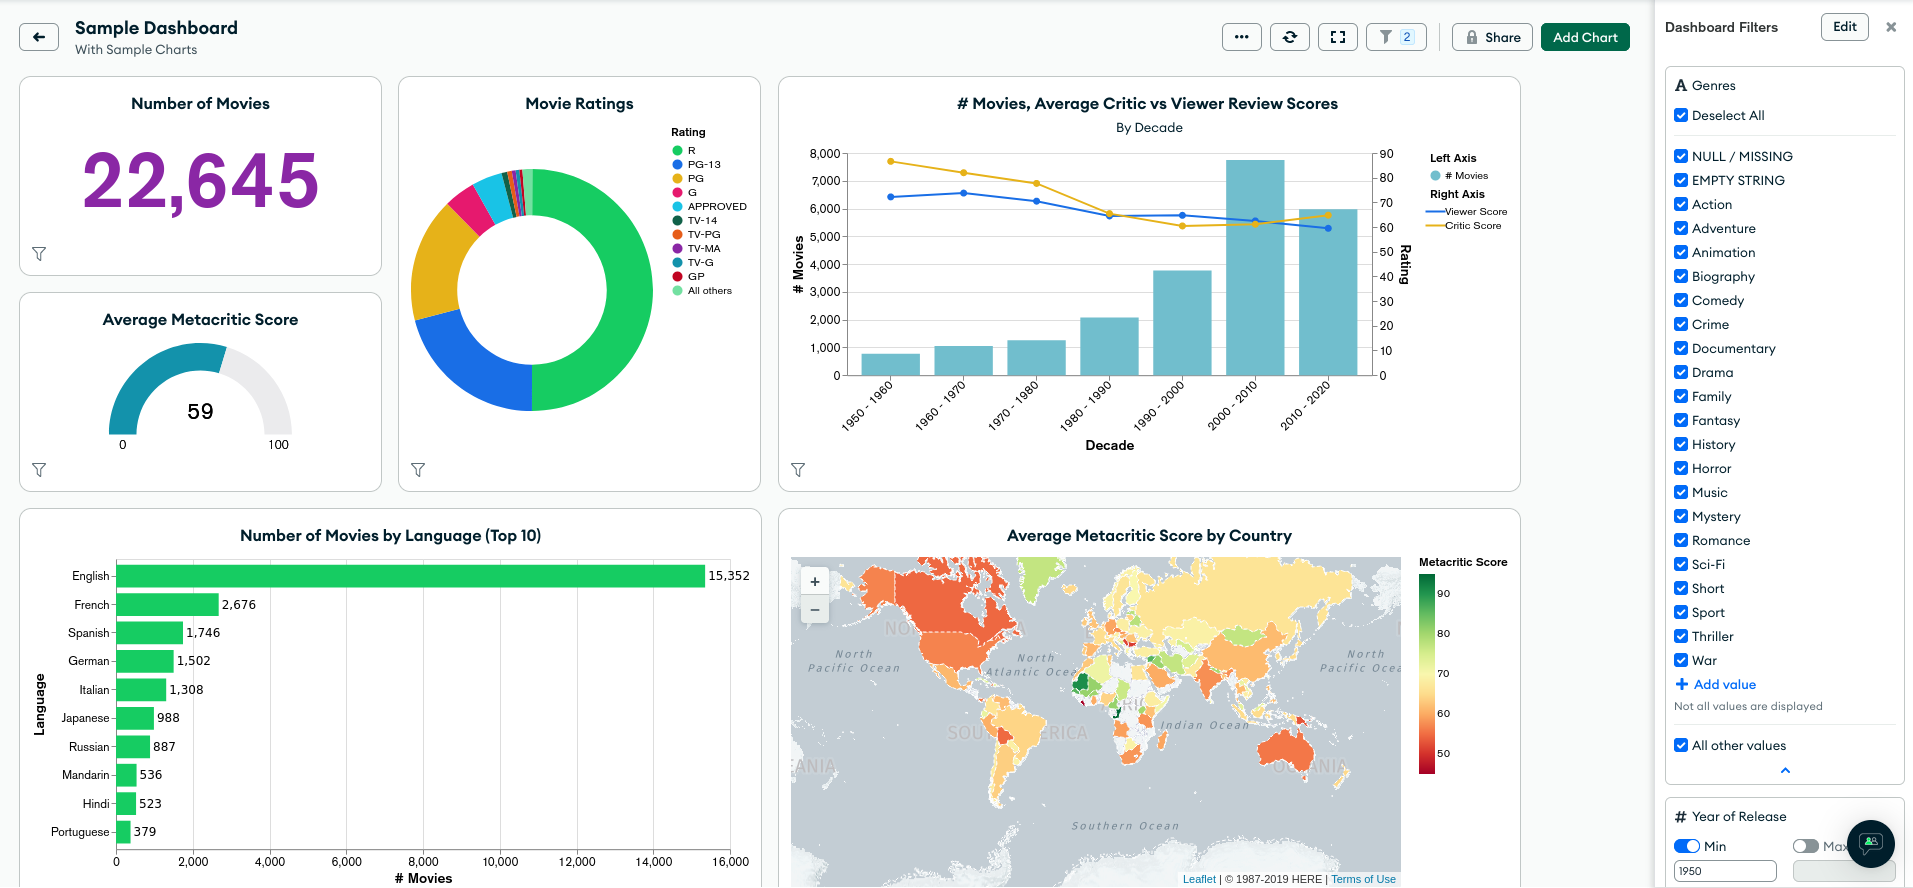
\includegraphics[width=\textwidth]{images/mongodb_charts}
    \caption{MongoDB Charts}
    \label{fig:mongodb_charts}
\end{figure}

\section{Verwendete Technologien}
\label{sec:verwendete_technologien}

\subsection{Backend Technologien}
\label{sec:verwendete_technologien_backend}

Da die Analyse der MongoDB Dokumente sehr rechenintensiv ist, wird die Analyse in ein Backend ausgelagert.
Um den zuvor definierten Anforderungen gerecht zu werden, ist es wichtig, ein geeignetes Backend-Framwork auszuwählen.
Das ER-Modellierungstool nutzt Java Spring als Backend-Framework.
Da man zum Teil Code von dem bestehenden Backend übernehmen könnte, bietet es sich deshalb an, in diesem Projekt ebenfalls Spring zu verwenden.

Für Spring gibt es eine MongoDB Implementierung namens Spring Data MongoDB.
Diese Implementierung ist jedoch dafür ausgelegt, \ac{pojo}s auf Dokumente zu mappen.
Im MongoDB Visualisierungstool sollen hingegen MongoDB Dokumente dynamisch eingelesen und analysiert werden.
Um ~\nameref{itm:ba2} zu erfüllen, ist es desweiteren nötig, beliebig viele verschiedene Datenbanken gleichzeitig zu verbinden und zu analysieren.
Die Verbindung mit MongoDB Datenbanken in Spring Data MongoDB erfolgt jedoch mit fixen Datenbanken, welche in der application.properties Datei definiert werden.
~\autocite{spring:spring-data-mongodb}
Deshalb ist die Spring Data MongoDB Bibliothek für diese Anwendung nicht geeignet.
Neben der Spring Data MongoDB Bibliothek gibt es auch noch einen anderen MognoDB Java Client, Java Sync.
Dieser funktioniert jedoch nicht zusammen mit dem Spring Framework.
Aus diesem Grund kann Spring sowie andere Java Backend Frameworks nicht genutzt werden.

Als alternatives Backend Framework mit REST Api bietet sich Flask an.
Ein großer Vorteil von Flask ist, dass Flask sehr minimal ist und nur mit dem minimum an benötigten Bibliotheken vorkonfiguriert ist.
Spring ist im Gegensatz dazu ein sehr mächtiges Framework mit vielen Features, von denen in diesem Projekt aber nur sehr wenige gebraucht werden.
Ein weiterer Vorteil von Flask sowie von Python ist die Schlankheit des Codes.
In Python lässt sich meist die gleiche Funktionalität in weniger Code schreiben als in Java.
Dazu kommt, dass in Flask sehr viel weniger Boilerplate Code benötigt wird als in Spring.
Ein minimaler Endpunkt in Flask lässt sich bereits mit 2 Zeilen Code umsetzen.
Zudem ist die dynamische Typisierung in Python beim Auswerten der MongoDB Dokumente von Vorteil, da man im Voraus nicht weiß, welche Datentypen die Werte in den Dokumenten haben, und die dynamische Typisierung deshalb das Handling dieser Werte vereinfacht.
~\autocite{khoirom2020comparative}

Jedoch hat Flask nicht nur Vorteile gegenüber Spring:
Flask ist grundsätzlich deutlich unperformanter als Spring.
Dies liegt unter anderem daran, dass Python eine interpretierte Sprache ist, und Java eine kompilierte.
~\autocite{sverker:rest_comparison}
Dies widerspricht zunächst der Anforderung ~\nameref{itm:ba1}.
Die Performance-Probleme lassen sich aber durch Multiprocessing ausgleichen.
Multiprocessing bedeutet, dass bestimmte Teile der Berechnung auf mehrere Threads im Prozessor aufgeteilt werden und dadurch parallell ausgeführt werden.
Python bietet eine simpel zu implementierende Lösung für Multiprocessing an, welche man bei der Analyse der Dokumente der MongoDB Datenbanken gut einsetzen kann.
Beispielsweise kann die Analyse jeder Collection von einem extra Thread ausgeführt werden.
Dadurch lässt sich die Anforderung ~\nameref{itm:ba1} mit Flask erfüllen.

In Python gibt es die Bibliothek PyMongo, welche alle der genannten Nachteile von Spring Data MongoDB ausbessert:
Mit PyMongo kann man direkt im Code beliebig viele MongoDB Datenbanken parallel dynamisch einbinden.
Mittels Objektorientierung lässt sich dadurch die parallele Analyse mehrerer Datenbanken sinnvoll umsetzen.
Zudem ist PyMongo nicht für das Mappen von Dokumenten auf Objekte gedacht.
Stattdessen kann man Dokumente als Python Dictionary auslesen.
Dies erleichtert die Analyse der Dokumente und hat darüber hinaus den Vorteil, dass man Dictionaries in Python in JSON umwandeln kann, was das Bauen der HTTP Response vereinfacht.
~\autocite{mongodb:pymongo}

\subsection{Frontend Technologien}
\label{sec:verwendete_technologien_frontend}

Web Apps haben gegenüber Desktop Apps einige Vorteile:
Web Apps müssen nicht installiert werden, sie müssen nicht für mehrere Betriebssysteme entwickelt werden und der Auslieferungs- Update- und Administrierungsprozess ist deutlich vereinfacht.
Jedoch haben Web Apps oftmals nicht die Interaktionsmöglichkeiten von Desktop Apps, da sie innerhalb eines Browsers laufen.
Dies ist in dieser Anwendung jedoch kein großer Nachteil, da die Hauptaufgabe der Anwendung die Visualisierung von Daten ist, und dies nicht viele Interaktionsmöglichkeiten erfordert.
~\autocite{zepeda2007desktop}
Deshalb wird das Frontend dieser Anwendung als Webapp entwickelt.

Das ER Modellierungstool benutzt das Frontend Framework React.
Da das ER Modellierungstool und das MongoDB Visualisierungstool Teil eines Datenbank Toolkits werden sollen, muss das MongoDB Visualisierungstool Frontend ebenfalls in React geschrieben werden, damit Anforderung ~\nameref{itm:fa1} erfüllt werden kann.
Da React dank React Elements und React Components in seiner Grundstruktur  sehr modular ist, eignet sich React sehr gut, um Anforderung ~\nameref{itm:fa2} zu erfüllen.
~\autocite{banks:react}
Die Tools lassen sich mittels Ordner strukturell voneinander trennen, und trotzdem können die Tools sich Komponenten teilen und diese wiederverwenden.

Dank der Komponentenbibliothek Material UI kann man in React vordefinierte Elemente benutzen, was oftmals das Definieren der Komponenten von Hand erspart.
Dadurch spart man sich einerseits Programmieraufwand, andererseits verringert dies aber auch die Code-Komplexität und verbessert somit die Lesbarkeit des Codes.
Zudem erleichtert Material UI das Umsetzen eines einheitlichen Designs, da man mithilfe von Material UI global verwendbare Themes erstellen kann.
Dies ermöglicht das Erfüllen der Anforderung ~\nameref{itm:fa5}.
~\autocite{mui:mui}

\section{REST-Schnittstelle}
\label{sec:rest_schnittstelle}
Das Backend stellt einen einzigen Endpunkt bereit: 
\textit{/connect} erwartet im Body des Requests folgende Daten im JSON-Format:
\begin{itemize}
    \item connection\_string: Der Connection String zur Verbindung mit der MongoDB Instanz
    \item database: Der Name der Datenbank, die analysiert werden soll
    \item analyse\_ref: True, wenn die Referenzen der Datenbank analysiert werden sollen
    \item sort\_method: Bestimmt, wie die Dokument-Variationen in einer Collection sortiert werden sollen
\end{itemize}
Mithilfe dieser Variablen versucht das Backend, sich mit der MongoDB Datenbank zu verbinden.
Wenn dies gelingt, wird die Datenbank ausgewertet und das Ergebnis als JSON im Response-Body zurückgegeben.
Wenn die Verbindung fehlschlägt, wird der Statuscode 406 zurückgegeben.

\section{Analyse der MongoDB Datenbank}
\label{sec:mongoDB_analyse}

Dokumente in MongoDB sind in einem JSON-Ähnlichen Format geschrieben.
Da man in Python JSON zu Dictionaries konvertieren kann, kann man mithilfe von PyMongo Dokumente als Dictionaries auslesen.
Dictionaries beinhalten eine Reihe an Key-Value Paaren.
Der Key entspricht dem Name des Feldes.
Aus dem Value kann man den Datentyp auslesen.
Ansonsten sind die Values nicht weiter von Relevanz, außer es handelt sich bei dem Datentyp um ein Array oder um einen Dictionary, also um ein verschachteltes Dokument.
In diesem Fall werden rekursiv wieder die Key-Value Paare aus dem entsprechenden Value ausgelesen. 
Die Ergebnisse dieser Analyse werden in einer Objektorientierten Datenstruktur gespeichert:
In der Klasse ProcessedCollection werden alle Variationen von Schemas gespeichert, inclusive dem Namen der Collection 
Die Schemas selber werden in der Klasse ProcessedDocument gespeichert incluive der Nummer an Dokumenten, die nach diesem Schema aufgebaut sind.
ProcessedDocument enthält wiederum eine Liste an Values.
Ein Value besteht aus einem Key, einem Typ, optional einer Referenz auf eine andere Collection (Wenn der Datentyp ObjectId ist und der Name nicht id\_ ist) und optional einem verschachtelten Dokument.

\begin{figure}[H]
    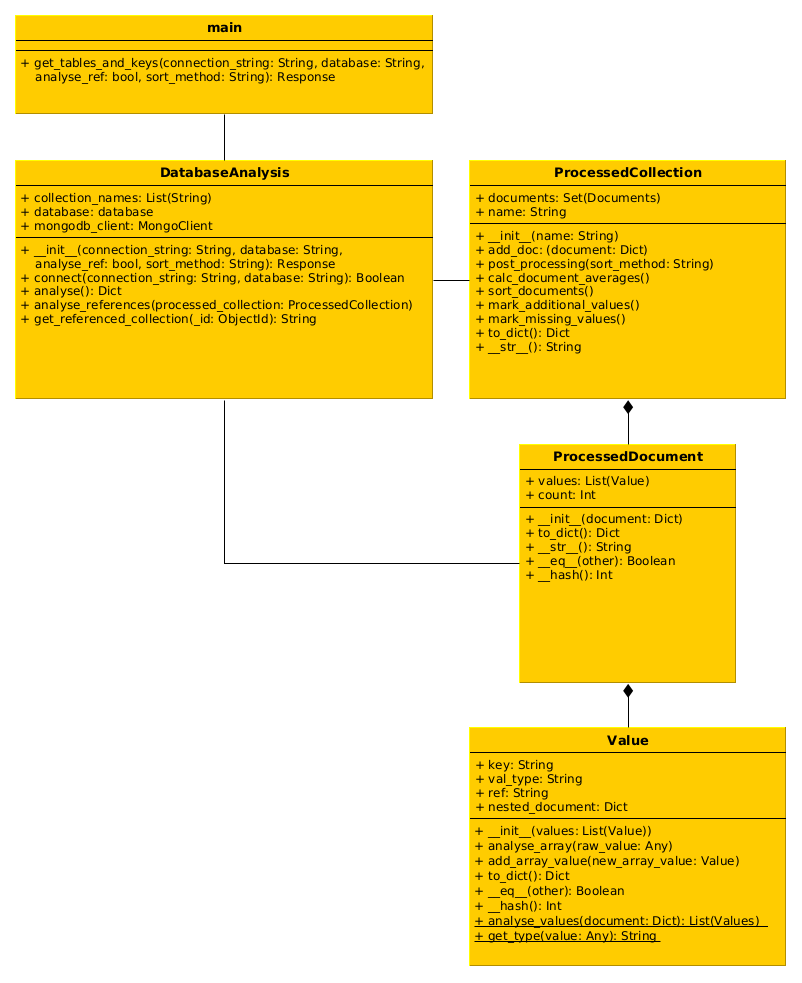
\includegraphics[width=\textwidth]{images/backend_uml}
    \caption{Backend UML Diagramm}
    \label{fig:backend_uml}
\end{figure}

\section{Planung des Frontends}
\label{sec:planung_frontend}

Um das Frontend zu planen, wurden in Miro, einem funktionsreichen Online-Whiteboard, Wireframes für die Screens des MongoDB Visualisierungstools gezeichnet.

Um ein einheitliches Layout und damit Anforderung ~\nameref{itm:fa5} zu gewährleisten, wird das gleiche Grundlayout wie in dem ER-Bildschirm des ER Modellierungstools verwendet.
Auf der linken Seite gibt es eine Left Sidebar, welche anstatt der ER-Elemente Verbindungsoptionen für die MongoDB Datenbank enthält. 
Der Hauptscreen in der Mitte zeigt nach erfolgreicher Verbindung die vom Backend extrahierten Hauptschemas jeder Collection als Tabellen an.
Diese Tabellen enthalten den Key, den Type und optional die referenzierte Collection.
Wenn der Datentyp Array oder Embedded Document ist, kann man eine Untertabelle aufklappen, welche die verschachtelten Daten enthält.


\begin{figure}[H]
    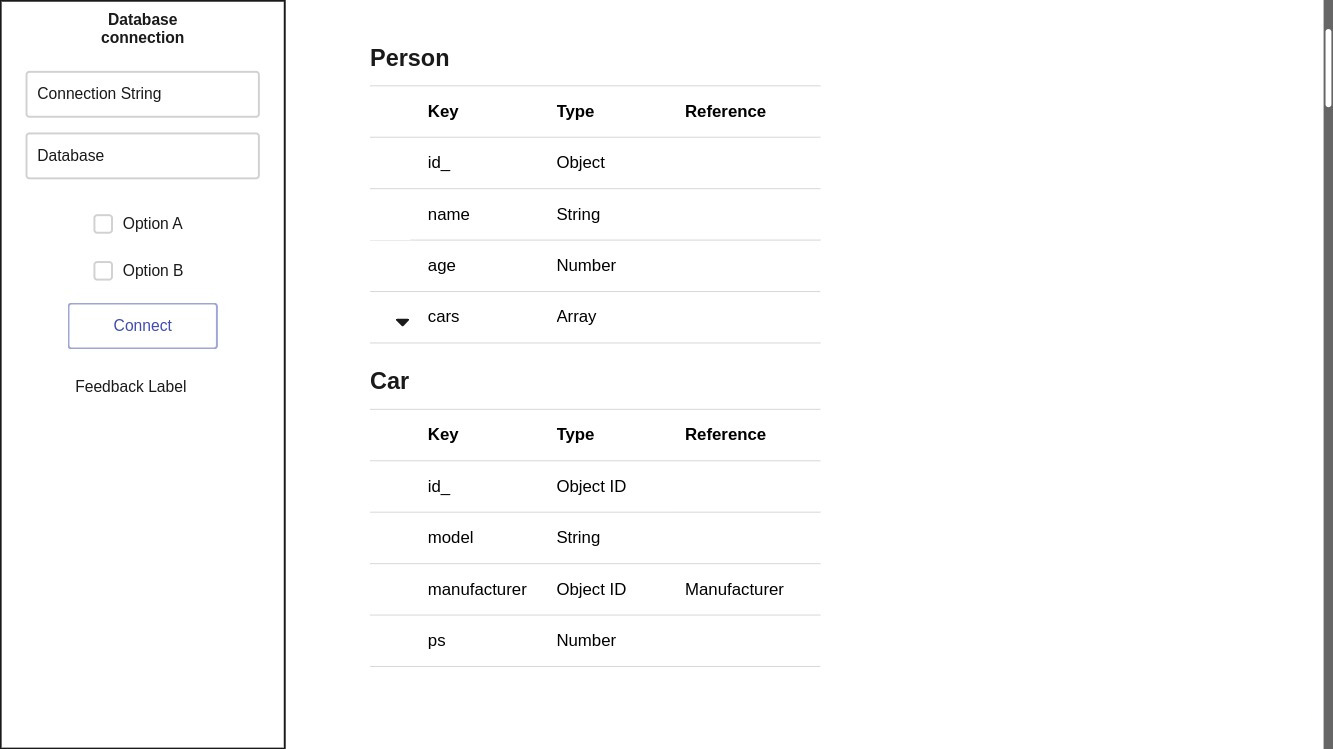
\includegraphics[width=\textwidth]{images/wireframe_vis_tool}
    \caption{Visualization Tool Wireframe}
    \label{fig:wireframe_vis_tool}
\end{figure}

Wenn man auf den Titel einer Tabelle in der Schema Übersicht klickt, öffnet sich die Detail View dieser Collection in einem Popup.
In dieser Detail View werden alle Variationen des Schemas angezeigt.
Zusätzliche Felder werden grün markiert, und fehlende in rot aufgelistet.
Zudem steht über jeder Schemavariation, von wie vielen Dokumenten diese Variation verwendet wird.

\begin{figure}[H]
    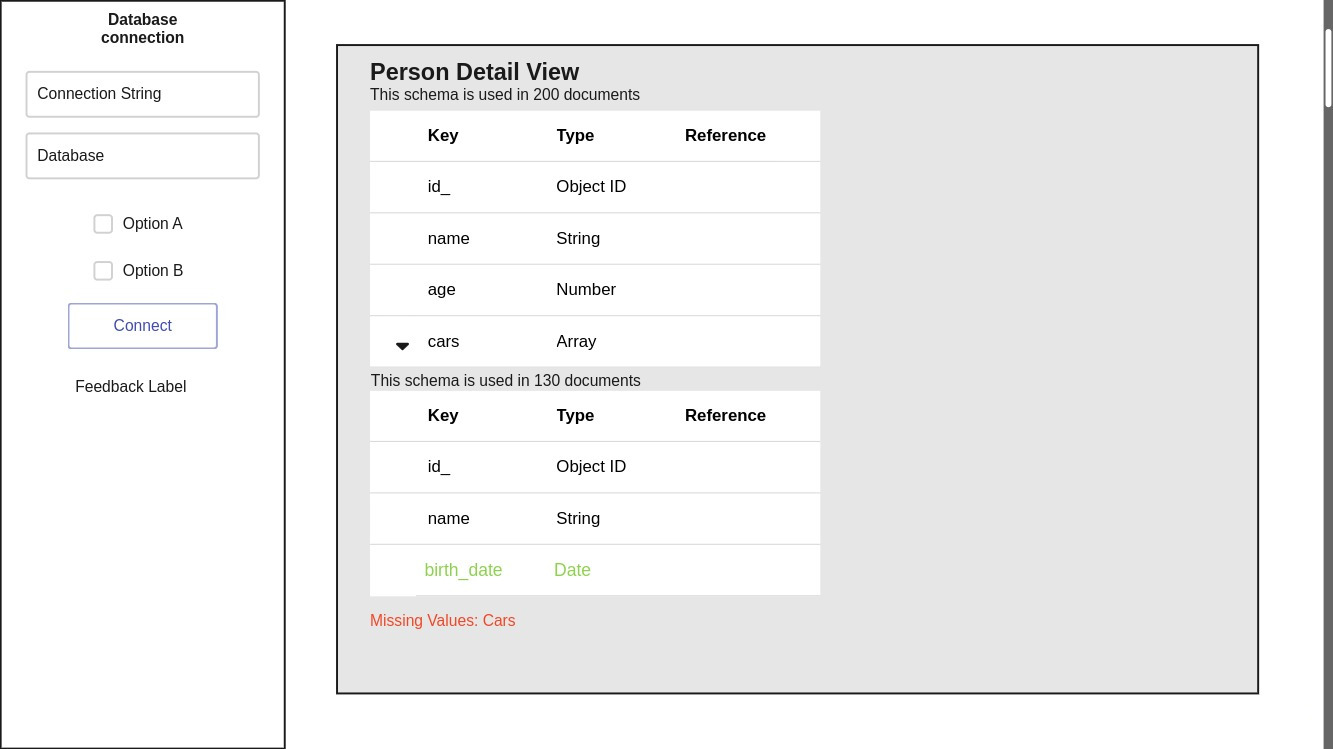
\includegraphics[width=\textwidth]{images/wireframe_detail_view}
    \caption{Detail View Wireframe}
    \label{fig:wireframe_detail_view}
\end{figure}

\section{Modularität des Frontends}
\label{sec:mod_frontend}

Um das Frontend Modular weiterbauen zu können, sind die Elemente im Components Package in ein Package pro Anwendung unterteilt.
Alle weiteren Packages werden Anwendungsübergreifend verwendet, sind also nicht weiter unterteilt.
Bei einer größeren Anzahl von Anwendungen könnten jedoch auch in diesen Packages Unterteilungen sinnvoll sein.

\begin{figure}[H]
    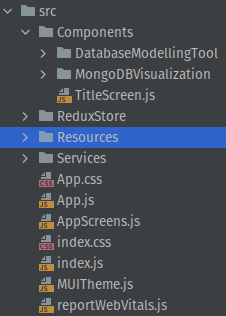
\includegraphics[width=\textwidth / 3]{images/frontend_package_structure}
    \caption{Frontend Package Structure}
    \label{fig:frontend_package_structure}
\end{figure}

Zudem wurde ein Titelbildschirm hinzugefügt, von welchem aus diese Anwendungen aufgerufen werden können.
Um eine neue Anwendung hinzuzufügen, muss man lediglich ein neues Package in Components erstellen und die benötigten Elemente anlegen, sowie im Titelbildschirm einen weiteren Button für die Anwendung hinzufügen.
